\section{Background}
\label{sec:background}

We now present the necessary background for this paper, largely following the terminology introduced in~\cite{chambers2023bounding}.

\subsection{Functors, Cosheaves and Mapper Graphs}
\label{sec:CategoryTheory}

We work in a category-theoretic setting and provide a brief overview of the necessary definitions, with more details provided in \cite{curry2013sheaves,riehl2017category}. 

A \emph{category} $\cC$ is a collection of objects $X,Y,Z,\dots$ along with morphisms $f,g,h,\dots$ such that 
\begin{enumerate}
    \item each morphism $f$ has a designated domain $X$ and codomain $Y$,
    \item every object has an identity morphism $\1_X\colon X \to X$,
    \item any pair of morphisms $f\colon X \to Y$ and $g\colon Y \to Z$ has a composite morphism $g \circ  f\colon X \to Z$ which satisfies an identity axiom, where $f\colon X \to Y = \1_Y \circ  f = f \circ \1_X$, and an associativity axiom, where $h\circ (g\circ f) = (h\circ g)\circ f$.
  \end{enumerate}
Many settings in mathematics can be viewed as categories: $\Set$ is the category whose objects are sets and morphisms are set maps; 
$\Top$ is the category whose objects are topological spaces and morphisms are continuous functions;
and, for a given topological space $X$, $\Open(X)$ is the category whose objects are the open sets and morphisms are given by inclusion. A category is \emph{small} if the collections of objects and morphisms are both sets.

Given two categories $\cC$ and $\cD$, a \emph{functor} $F\colon\cC \to \cD$ maps each object $x \in \cC$ to an object $F(x) \in \cD$ and each morphism $f\colon X \to Y$ to a morphism $F[f]\colon F(X) \to F(Y)$ that satisfies the following properties: for any $X \in \cC$, $F[\1_X] = \1_{F(X)}$; for any $f,g \in \cC$ for which the composition $gf$ is defined, we have $F[gf] = F[g] F[f]$. 
Given two functors $F,G\colon \cC \to \cD$, a \emph{natural transformation} $\eta\colon F \Rightarrow G$ is a collection of maps $\eta_X\colon F(X) \to G(X)$ such that for any morphism $f\colon X \to Y$ in $\cC$, the diagram 
\begin{equation*}
\begin{tikzcd}
X\ar[d,  "f"] 
& F(X) 
    \ar[r, "\eta_X"] 
    \ar[d, "{F[f]}"']
& G(X) 
    \ar[d, "{G[f]}"]
\\
Y 
& F(Y) \ar[r, "\eta_Y"] 
& G(Y)
\end{tikzcd}
\end{equation*}
commutes. 
One example of a functor is $\pi_0\colon\Top \to \Set$, where $\pi_0(X)$ denotes the set of path-connected components of a topological space $X$, and the morphisms are set maps $\pi_0[f]\colon \pi_0(X) \to \pi_0(Y)$ sending a path-connected component $A$ in $X$ to the element $f(A)$ in $Y$.

In the special case where $J$ is a small category, a diagram is simply a functor $F\colon J \to \cC$.
Let $c \in \cC$. By a slight abuse of notation, we define the constant functor $c \colon J \to \cC$, $c(j) \mapsto c$ for all $j \in J$ and all morphisms are sent to the identity morphism. 
In this setting, a \emph{cocone} is a natural transformation $\lambda\colon F \to c$.
We denote $\lambda_j\colon F(j) \to c$ 
%
and note that for any $f\colon j \to k$ in $J$, $\lambda_k \circ F[f] = \lambda_j$. 
A cocone $\lambda\colon F \to c$ is a \emph{colimit} if, for any other cocone $\lambda'\colon F \to c'$, there is a unique  morphism $u\colon c \to c'$ such that the diagram
\begin{equation*}
\begin{tikzcd}
F(j) 
    \ar[rr, "{F[f]}"]
    \ar[dr, "\lambda_j"]
    \ar[ddr, "\lambda_j'"']
&& F(k)
    \ar[dl, "\lambda_k"']
    \ar[ddl, "\lambda_k'"]
\\
& c \ar[d, dashed, "u"] \\
& c'
\end{tikzcd}
\end{equation*}
commutes for all $f\colon j \to k$ in $J$. 
We denote this by $\colim_I(F)$, and note that this always exists and is unique in our setting where $\cD =\Set$.

For the rest of this paper, we turn our attention to functors of the form $F\colon\Open(X) \to \Set$, called \emph{pre-cosheaves}. 
We are particularly interested in the case when a pre-cosheaf is a \emph{cosheaf}. In short, a cosheaf is a presheaf that is entirely and uniquely defined by any open cover of ${U \in \Open(X)}$.
More rigorously, given an object $U \in \Open(X)$ and a cover $\{U_\alpha\}_{\alpha \in A}$ of $U$, define a category $\cU = \{U_\alpha \cap U_{\alpha'} \mid \alpha,\alpha' \in A \}$ with morphisms given by inclusion. As these open sets $U_\alpha$ are themselves objects in $\Open(X)$, the functor $F\colon\cU \to \Set$ is well-defined, so we can consider its colimit $\lambda\colon F \to L$. A \emph{cosheaf} is a functor $F$ whose unique map $L \to F(U)$ given by the colimit definition is an isomorphism for every $U \in \Open(X)$.


%



%
%
%
%
%


%
%
%
%

%
%




%
%
%
%
%
%
%
%
%
 

\subsection{Mapper Cosheaves and the Interleaving Distance}
\label{ssec:functorGraphs}

In this section, we show how we can represent the data of a mapper graph as a cosheaf. 
We assume that we are given data in the form of a compact topological space with a function $f\colon\X \to \R$. 
Fix a resolution $\delta>0$. 
We assume $\Im(f) \subseteq[-\delta L, \delta L]$.
This choice of resolution induces a discretization of $[-\delta L, \delta L]$ into a cell complex $K$ where the 0-cells are given by the points $\{ \sigma_i \coloneqq i \delta \mid i \in [-L, \cdots,L]\}$, and edges are given by the intervals $\{ \tau_i \coloneqq (i \delta, (i+1)\delta) \mid i  \in [-L, L-1] \}$. Further, $K$ induces a cover of the image with cover elements of the form 
%
    \[\{ U_{\sigma_i} = ((i-1)\delta, (i+1)\delta) \mid i \in \{-L+1,\cdots, L-1\}\} \]
%
and intersections of the form
%
    \[\{ U_{\tau_i} = (i\delta, (i+1)\delta) \mid i \in [-L,\cdots, L-1]\}.\]
%
Together, we write $\cU= \{U_{\sigma_i}\} \cup \{ U_{\tau_i}\}$. 
The set $\cU$ forms a poset $(\cU, \subseteq)$ under inclusion. 
We use $\rho \in K$ to denote either a $\sigma_i$ or a $\tau_i$, and similarly write $U_\rho \in \cU$ when referring to cells of either dimension.

We define open sets in this poset using the Alexandrov topology, following \cite{Barmak2011} and \cite{chambers2023bounding}.
Given this poset $(\cU,\subseteq)$, for any set $S \subseteq \cU$, the upset is 
$S^{\uparrow} = \{U \in \cU \mid \exists \,V \in S,\, V \subseteq U  \,  \}$ 
and the downset is
$S^{\downarrow} = \{ U \mid \exists\,  V \in S,\, U \subseteq V \}$. 
A set $S \subset \cU$ is said to be open iff $S^{\downarrow} = S$ or equivalently, if for any $U \in S$, and any $V \subset U$, $V \in S$. 
It can be checked that this topology has a basis given by the set of downsets: 
write $S_\rho = \{ U_{\rho}\}^{\downarrow}$, then the basis for $\Open(\cU)$ is given by $\{ S_\rho^{\downarrow} \mid \rho \in K\}$ and we call $S_\rho$ a basic open set. 
See the left of \cref{fig:PosetNotation} for a visualization of this notation. 

We will often use these combinatorial subsets of $\cU$ interchangeably with their geometric realizations, given by $|S| \coloneqq \bigcup_{U \in S} U \subset \R$. 
We can check that this notation is then reasonable on our  set. 
First, for $\sigma_i = i \delta$ and $U_{\sigma_i} = ((i-1)\delta, (i+1)\delta) \subset \R$, we have 
${\{U_{\sigma_i}\}^{\downarrow} =\{U_{\tau_i},U_{\sigma_i},  U_{\tau_{i+1}}\}}$ 
and $|\{U_{\sigma_i}\}^{\downarrow}| = U_{\sigma_i}$. 
Similarly, for $U_{\tau_i} = (i\delta, (i+1)\delta)$, 
$\{U_{\tau_i}\}^{\downarrow} =\{U_{\tau_i}\} $, and of course 
$|\{U_{\tau_i}\}^{\downarrow}| = U_{\tau_i}$.
Again, see \cref{fig:PosetNotation} for an illustration of the notation. 

\begin{figure}
    \centering
    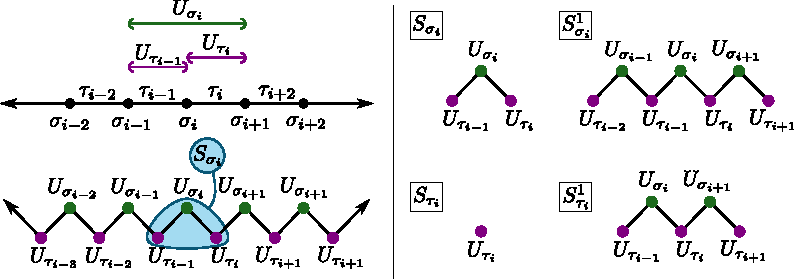
\includegraphics[width=\textwidth]{figures/MapperCoverPosetv2.pdf}
    \caption{The notation for the cover of $\R$. Left: the distinction between the cover element $U_{\sigma}$ and the open set in the Alexandrov topology, $S_{\sigma}$, which is a discrete set of three objects. Right: 1-thickenings $S_{\sigma_i}$ and $S_{\tau_i}$ for the two types of basis open sets. (Left side of figure modified from \cite{chambers2023bounding}). } 
    \label{fig:PosetNotation}
\end{figure}

Let $\pi_0\colon \Top \to \Set$ denote the functor returning the set of path connected components of a given topological space. 
Then the mapper cosheaf of $(\X,f)$ at resolution $\delta$ is given by the functor 
\begin{equation*}
\begin{matrix}
    F\colon & \Open(\cU) & \rightarrow & \Set \\
       & S & \mapsto & \pi_0(f\inv(|S|))
\end{matrix}
\end{equation*}
By functoriality of $\pi_0$, for open sets $S \subseteq T$, $F$ induces a map
\[F[S \subseteq T] \colon \pi_0f\inv(|S|) \to \pi_0f\inv(|T|),\]
so that $F$ satisfies the requirements of being a functor.
Furthermore, this functor satisfies the definition of a cosheaf. 
Thus, we call any cosheaf of the form $F\colon \Open(\cU) \to \Set$ a \textit{mapper cosheaf}. 
For notational simplicity, we write the induced map as $F[\subseteq]\colon F(S) \to F(T)$ when $S \subseteq T$ is clear from context. 

We next show that we can define an interleaving on these mapper cosheaves.
Given any open set $S \in \Open(\cU)$, we construct the \emph{1-thickening} by taking the downset of the upset of $S$, denoted by
$S^1 = (S^{\uparrow})^\downarrow$.
The \emph{$n$-thickening} is defined to be $n$ repetitions of this process, given recursively as
\begin{equation*}
    S^n = 
    \begin{cases}
    S & n = 0;\\
    (S^{n-1})^{\uparrow\downarrow} & n \geq 1.
    \end{cases}
\end{equation*}
Each $S^n$ is an element of $\Open(\cU)$, if $S \subseteq T$, then $S^n \subseteq T^n$. 
Thus we can view the thickening operation as a functor $(-)^n\colon \Open(\cU)   \to   \Open(\cU)$.
It is easy to check  that for a basic open $S_{\sigma_i}$, $|S_{\sigma_i}^n| = ((i-n)\delta, (i+n)\delta)$ and for $S_{\tau_i}$, $|S_{\tau_i}^n| = ((i-n)\delta, (i+1+n)\delta)$. 
See the right of \cref{fig:PosetNotation} for an example of 1-thickenings of basic opens.

As shown in previous work \cite{chambers2023bounding}, this thickening can be used to define an interleaving distance that compares mapper cosheaf functors  
${F,G\colon\Open(\cU) \to \Set}$.
We use $F^n$ to denote the composition of functors $F \circ ( - )^n\colon \Open(\cU) \to \Set$, so that $F^n(S) = F(S^n)$, and similarly for $G^n$. 
We define an \emph{$n$-interleaving} to be a pair of natural transformations $\phi\colon F \Rightarrow G^n$ and $\psi\colon G \Rightarrow F^n$ given by set maps $\phi_S\colon F(S) \to G(S^n)$. 
We note the map at $S^n$, $\phi_{S^n}\colon F(S^n) \to G(S^{2n})$, can also be viewed as a component map of a natural transformation $\phi^n\colon F^n \Rightarrow G^{2n}$. Therefore, when $\phi$ is indeed a natural transformation, we use the notation $\phi_{S^n}$ and $\phi_S^n$ interchangeably.


\begin{definition}[\cite{chambers2023bounding}]
\label{def:interleavingDistance}
Let $F,G\colon\Open(\cU) \to \Set$ be cosheaves and $n \in \mathbb{Z}_{\geq 0}$. An \emph{$n$-interleaving} is a pair of natural transformations 
$\phi\colon F \Rightarrow G^n$
and 
$\psi\colon G \Rightarrow F^n$
such that the diagrams 
\begin{equation*}
    \begin{tikzcd}[ampersand replacement=\&]
        F(S) 
            \ar[rr, "{F[S \subseteq S^{2n}]}"]   
            \ar[dr, "\phi_S"',violet] 
            \& \& F(S^{2n}) \& 
        \& F(S^n) \ar[dr]
            \ar[dr, "\phi_{S^{n}}",violet]
        \& \\
        \& G(S^n)\ar[ur, "\psi_{S^n}"', orange]  \& \& 
        G(S) 
            \ar[rr, "{G[S \subseteq S^{2n}]}"']
            \ar[ur, "\psi_{S}", orange]  
        \&\& G(S^{2n})
    \end{tikzcd}
\end{equation*} 
commute for all $S \in \Open(\cU)$.
The \emph{interleaving distance} is given by 
\begin{equation*}
    d_I(F,G) = \inf\{ n \geq 0 \mid \text{there exists an $n$-interleaving} \}, 
\end{equation*}
and is set to be $d(F,G) = \infty$ if there is no interleaving for any $n$.
\end{definition}

For the sake of simplicity, we will denote these diagrams by $\triangled_{\phi,\psi}(S)$ and $\triangleu_{\phi,\psi}(S)$, respectively. Similarly, we denote the diagrams representing natural transformations
\begin{equation*}
    \begin{tikzcd}
        F(S)  
            \ar[r, "{F[\subseteq ]}"] 
            \ar[dr, "\phi_S"', very near start, violet]
        & F(T)
            \ar[dr, "\phi_T"', very near start, violet]
        & \\
        & G(S^n) 
            \ar[r, "{G[\subseteq ]}"'] 
        & G (T^n)
    \end{tikzcd}
    \hspace{1cm}
    \begin{tikzcd}
        & F(S^n)
            \ar[r, "{F[\subseteq ]}"] 
        & F (T^n)\\
        G(S)
            \ar[r, "{G[\subseteq ]}"'] 
            \ar[ur, "\psi_S", very near start, orange]
        & G(T) 
            \ar[ur, "\psi_T", very near start, orange]
        & 
    \end{tikzcd}
\end{equation*}
by $\Parallelograml_\phi(S,T)$ and $\Parallelogramr_\psi(S,T)$, respectively. 
As shown in \cite{chambers2023bounding}, \cref{def:interleavingDistance} fits in the interleaving framework built by Bubenik et al.~\cite{bubenik2015metrics} and thus it is an extended pseudometric.

%
\subsection{Loss Function Definition}
\label{ssec:LossFunction}

In this section, we outline the loss function, largely following \cite{chambers2023bounding}, with some necessary technical modifications.
First, we introduce the notion of an assignment, inspired by~\cite{Robinson2020} and~\cite{nlab:unnatural_transformation}, which we use to denote collections of morphisms used to define an interleaving, without requiring that these morphisms form a natural transformation.

\begin{definition}[Modified from \cite{chambers2023bounding}]
\label{def:assignment}
Given functors $H,H'\colon\Open(\cU) \to \Set$, an \emph{unnatural transformation}\footnote{A  natural transformation is an unnatural transformation which obeys commutativity properties, so the two sets are not mutually exclusive.}   $\eta\colon H \rightarrow H'$ is a collection of maps $\eta_S\colon H(S) \to H'(S)$ with no additional promise of commutativity. 
For a fixed $n \geq 0$ and cosheaves $F$ and $G$, an \emph{$n$-assignment} is a pair of unnatural transformations $\phi\colon F \Rightarrow G^n$ and $\psi\colon G \Rightarrow F^n$.

An \emph{(extended) basis unnatural transformation} 
$\eta\colon H \leadsto (H')^n$ for mapper cosheaves $H$ and $H'$ is a collection of maps
\begin{equation*}
    \eta = \{ \eta_{S_\rho}\colon H(S_\rho) \to H'(S_\rho^n) \mid \rho \in K\} 
        \cup \{\eta_{S_\rho^n}\colon H(S_\rho^n) \to H'(S_\rho^{2n}) \mid \rho \in K\}
\end{equation*}
for all basis elements $S_\rho$ from $\rho \in K$. 
A \emph{basis $n$-assignment} (or simply a \emph{basis assignment}) is a pair of extended basis unnatural transformations
$
\phi\colon F \leadsto G^n
$
and 
$
\psi\colon G \leadsto F^n.
$
\end{definition}
The modification from \cite{chambers2023bounding} presented here is to include the maps $\eta_{S^n_\sigma}$ along with $\eta_{S_\sigma}$ as part of the basis $n$-assignment. 
In \cite{chambers2023bounding}, we used the fact that the maps $\eta_{S_\sigma}$ could be used to determine $\eta_{S^n_\sigma}$; however the matrix representations introduced in \cref{sec:DataStructure} do not allow for easy computation of this extension. 
Thus, we have modified the definition so that the maps $H(S_\sigma^n) \to H(S_\sigma^{2n})$ are also given as input. 
For the remainder of the paper, we use the term ``basis unnatural transformation'' to imply the extended definition given here. 

We take these basis unnatural transformations and extend them to natural transformations after a shift using a value $k$.
We adopt the following notation:
when an assignment might not commute, we  denote its maps by lower case $\phi \colon F \leadsto G^n$ and $\psi\colon G \leadsto F^n$ with squiggly arrows; for assignments which are constructed to be natural transformations, we  denote them by upper case $\Phi\colon F \Rightarrow G^n$ and $\Psi\colon G \Rightarrow F^n$ with double arrows. 
\begin{definition}[\cite{chambers2023bounding}]
\label{def:extend_unnat_trans}
Given a basis unnatural transformation $\phi\colon F \leadsto G^n$ and a fixed $k$, define the (non-extended) basis unnatural transformation $\Phi\colon F \Rightarrow G^{n+k}$ by 
$\Phi_S =  G[S^n \subseteq S^{n+k}] \circ \phi_S$
for all $S \in \{S_\sigma \mid \sigma \in K\}$. %
\end{definition}

We measure the quality of an  $n$-assignment $\phi, \psi$ using  collections of distances for all open sets, $\{d_S^F \mid S \in \Open(\cU)\}$ and $\{d_S^G \mid S \in \Open(\cU)\}$, defined as follows.  
\begin{definition}[\cite{chambers2023bounding}]
The distance $d_S^{F}(A,B)$ for $A,B \in F(S)$ is defined to be 
\begin{equation}
\label{eqn:DistanceDefinition}
    d_S^{F}(A,B) = 
    \min\{ k\geq0 \mid F[S \subset S^k](A) = F[S \subset S^k](B)\}.
\end{equation}
If no such $k$ exists, then we  set $d_S^{F}(A,B) = \infty$.
\end{definition}
Geometrically, this can be thought of as the smallest integer $n$ such that the connected components represented by $A$ and $B$ in $f\inv(|S|)$ are in the same connected component when included into $f\inv(|S^n|)$. 
Further, we can see that this distance is an ultrametric since if for ${A,B,C \in F(S)}$, $k = \max\{d_S^{F}(A,B), d_S^{F}(B,C)\}$, then $A$, $B$, and $C$ all map to the same object in $F(S^k)$, and thus $d_S^F(A,C) \leq k$. 
\begin{definition}[\cite{chambers2023bounding}]
\label{df:Loss_by_diagram}
Fix an $n$-assignment
$(\phi,\psi)$. 
We define four \emph{diagram loss functions}: 
\begin{align*}
\Lpl^{S,T}(\phi)
    &= \max\limits_{\alpha \in F(S)} 
       d_{T^n}^{G}(
        \varphi_T \circ F[S \subseteq T](\alpha),
        G[S^n \subseteq T^n] \circ \varphi_S(\alpha)
        );\\
\Lpr^{S,T} (\psi)
    &= \max\limits_{\alpha \in G(S)} 
       d_{T^n}^{F}(
        \psi_T \circ G[S \subseteq T](\alpha), 
        F[S^n \subseteq T^n] \circ \psi_S(\alpha)
    );\\
\Ltd^S (\phi,\psi)
    &= \max\limits_{\alpha \in F(S)}  \Big \lceil \tfrac{1}{2} \cdot d_{S^{2n}}^{F}(
    F[S \subseteq S^{2n}] (\alpha),
    \psi_{S^n} \circ \varphi_S(\alpha)
    ) \Big \rceil;\\
\Ltu^S (\phi,\psi)
    &= \max\limits_{\alpha \in G(S)}\Big \lceil \tfrac{1}{2} \cdot d_{S^{2n}}^{G}(
    G[S \subseteq S^{2n}](\alpha),
    \varphi_{S^n} \circ \psi_S(\alpha)
    )\Big \rceil.
\end{align*}
\end{definition}
Combining these ideas, we define the loss function between given $n$-assignments.

\begin{definition}[Modified from \cite{chambers2023bounding}]
\label{shortdef}
Given an $n$-assignment $(\phi,\psi)$, the \emph{(extended basis) loss function} is 
\begin{equation}
\label{eq:loss}
L_B(\phi,\psi) = \max_{ \substack{\sigma < \tau \in K \\ \rho \in K}}
\left\{
\Lpl^{S_\tau, S_\sigma}, \Lpr^{S_\tau, S_\sigma},
\Lpl^{S_\rho, S_\rho^n}, \Lpr^{S_\rho, S_\rho^n},
\Ltu^{S_\rho}, \Ltd^{S_\rho}
\right\}
\end{equation}
where the max is over all cells $\rho \in K$ of any dimension, or adjacent edge-vertex pairs $(\tau, \sigma)$. 
\end{definition}

Again, note the slight modification from the definition given in  \cite{chambers2023bounding} where two additional terms, $\Lpl^{S_\rho, S_\rho^n}$ and $\Lpr^{S_\rho, S_\rho^n}$, are included in this new loss function. 
Because the extended basis unnatural transformation provides the maps 
$\phi_{S_\sigma^n}\colon F(S_\sigma^n) \to G(S_\sigma^{2n})$ as inputs rather than being determined from the maps $\phi_{S_\sigma}$, we are taking a maximum over more inputs so it is an immediate corollary that this function gives a bound on the true interleaving distance. 

\begin{theorem}[{Corollary of \cite[Theorem 3.16]{chambers2023bounding}}]
\label{maintheorem}
Given an (extended) basis $n$-assignment  
$\phi$
and 
$\psi$, 
we have 
$d_I(F,G) \leq n + L_B(\phi,\psi).$
\end{theorem}
